\chapter{Conclusion and Future Work}\label{conclusionfuturework}
This chapter concludes this Master's Thesis and offers an outlook for possible
future work based on the experiences gained throughout.

The integration of \ac{UML} profiles into the SiDiff and SiLift tools has
succesfully been achieved in this Master's Thesis. For the whole pipeline to
work with such profiled models all parts had to be adapted, namely:
\begin{itemize}
  \item Matching
  \item Lifting
  \item Patching
\end{itemize}
All three parts have successfully been adapted, whereas three new services and
tools have been introduced in this thesis:
\begin{itemize}
  \item \textbf{ProfileMatcher}\\
  		This services integrates \ac{UML} profiles into SiDiff and therefore allows
  		matching of such.
  \item \textbf{\ac{UUID}Fixer}\\
  		This new service allows for fixing of wrong identifiers and can be used for
  		compliance of models to other modeling tools.
  		\newpage
  \item \textbf{ProfileApplicator}\\
  		This new tool integrates \ac{UML} profiles into SiLift and therefore
  		lays the foundation for the lifting and patching functionalities.
\end{itemize}
After
the integration process in the course of this Master's Thesis the results have
been tested using a real world \ac{SysML} case study. First one example has
been introduced in detail and has been tested followed by a batch patch
application testing all revision of the whole case study. The final
result achieved is the successful  integration of \ac{UML} profiles as all tools
deliver the expected results, especially the final test for equality between
patched models and their corresponding revisions. The newly integrated support
for \ac{UML} profiles into SiDiff and SiLift increases their support of modeling
domains drastically, as many new modeling domains may arise by the aid of the
implemented profiling mechanism. Additionally the real world case study
created in \ac{SysML} can be used in future tools in this ecosystem, as it
represents a complex model and can be utilized for runtime tests for example.
The newly adapted \ac{UML} configuration for SiDiff can be used in other
contexts as well. A final overview of the results achieved in this Master's
Thesis are presented in figure~\ref{intergration_result_overview}.

 \begin{figure}[h!]
\begin{center}
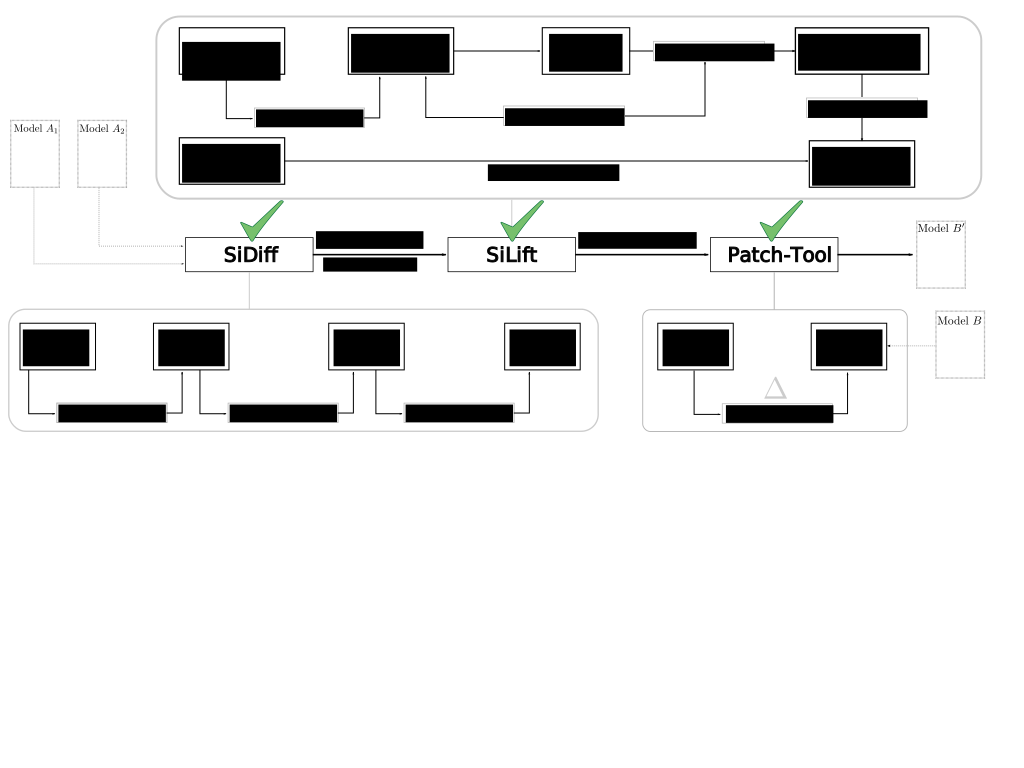
\includegraphics[scale=0.5]{integration_overview_ready_p6}\\
\end{center}
\caption{Final integration result overview}
\label{intergration_result_overview}
\end{figure}
\newpage
The following aspects could be considered in future work:
\begin{itemize}
  \item \textbf{Testing of other profiles}\\
  		Additionally to the tested \ac{UML} profile \ac{SysML} others like
  		\ac{MARTE} can be used for testing, as their results may differ.
  		\ac{MARTE} makes use of own semantics in stereo types which needs to be adressed explicitly. One solution is the addition of
  		a new compare method for SiDiff which takes the similarity of stereo typed
  		elements into consideration.
  \item \textbf{Construction of edit rules}\\
 		To achieve better lifting result one can define more complex edit rules
 		than defined in this Master's Thesis for \ac{UML} itself or for a given
 		profile.
  \item \textbf{Implement remaining variants}\\
  		As in this Master's Thesis only variant 3 of the different integration
  		approaches into SiLift has been implemented, both remaining could be
  		implemented in the future. As depicted in figure~\ref{variants_overview} the
  		first variant would result in an integration into \ac{SERGe}, whereas the
  		second variant shall be implemented as own tool. Instead of supporting only
  		the merging of base and profiled edit rules one can implement such Henshin
  		rule merger generically and therefore support the merging of Henshin rules
  		in general. This would result in new possibilities like merging two atomic
  		edit rules into one complex rule without the need of manual intervention.
  \item \textbf{Performance optimizations}\\
  		As the newly supported \ac{SysML} case study can be described as complex,
  		some parts in the tooling pipeline shall be taken into consideration for
  		performance optimizations. This concerns elements like runtime or memory
  		consumption as well as user interface optimizations.
\end{itemize}